\documentclass[9pt,twocolumn,twoside,]{pnas-new}

% Use the lineno option to display guide line numbers if required.
% Note that the use of elements such as single-column equations
% may affect the guide line number alignment.


\usepackage[T1]{fontenc}
\usepackage[utf8]{inputenc}

% tightlist command for lists without linebreak
\providecommand{\tightlist}{%
  \setlength{\itemsep}{0pt}\setlength{\parskip}{0pt}}


% Pandoc citation processing
%From Pandoc 3.1.8
% definitions for citeproc citations
\NewDocumentCommand\citeproctext{}{}
\NewDocumentCommand\citeproc{mm}{%
  \begingroup\def\citeproctext{#2}\cite{#1}\endgroup}
\makeatletter
 % allow citations to break across lines
 \let\@cite@ofmt\@firstofone
 % avoid brackets around text for \cite:
 \def\@biblabel#1{}
 \def\@cite#1#2{{#1\if@tempswa , #2\fi}}
\makeatother
\newlength{\cslhangindent}
\setlength{\cslhangindent}{1.5em}
\newlength{\csllabelwidth}
\setlength{\csllabelwidth}{3em}
\newenvironment{CSLReferences}[2] % #1 hanging-indent, #2 entry-spacing
 {\begin{list}{}{%
  \setlength{\itemindent}{0pt}
  \setlength{\leftmargin}{0pt}
  \setlength{\parsep}{0pt}
  % turn on hanging indent if param 1 is 1
  \ifodd #1
   \setlength{\leftmargin}{\cslhangindent}
   \setlength{\itemindent}{-1\cslhangindent}
  \fi
  % set entry spacing
  \setlength{\itemsep}{#2\baselineskip}}}
 {\end{list}}
\usepackage{calc}
\newcommand{\CSLBlock}[1]{#1\hfill\break}
\newcommand{\CSLLeftMargin}[1]{\parbox[t]{\csllabelwidth}{#1}}
\newcommand{\CSLRightInline}[1]{\parbox[t]{\linewidth - \csllabelwidth}{#1}\break}
\newcommand{\CSLIndent}[1]{\hspace{\cslhangindent}#1}

\usepackage{graphicx}
\setkeys{Gin}{height=0.75\textheight,keepaspectratio}
\renewcommand{\significancestatement}[1]{}
\date{}
\makeatletter \def\@isdraft{0} \makeatother
\makeatletter \def\watermark{} \makeatother
\PassOptionsToPackage{nopatch=eqnum}{microtype}

\templatetype{pnasresearcharticle}  % Choose template

\title{Analyse de viabilité de population de la situation du Chevalier
Cuivré (\emph{Moxostoma hubbsi}) en utilisant une matrice de Lefkovitch
à 3 stades}

\author[a]{Tristan Plasse}
\author[a]{Yohan Wegener}

  \affil[a]{Université de Sherbrooke, Département de Biologie,
Sherbrooke, Québec, J1K 2R1}


% Please give the surname of the lead author for the running footer
\leadauthor{}

% Please add here a significance statement to explain the relevance of your work
\significancestatement{}


\authorcontributions{}



\correspondingauthor{\textsuperscript{} }

% Keywords are not mandatory, but authors are strongly encouraged to provide them. If provided, please include two to five keywords, separated by the pipe symbol, e.g:


\begin{abstract}
Ce travail s'inscrit dans la continuité des recherches portant sur
l'état de la population du Chevalier cuivré (Moxostoma hubbsi), une
espèce endémique du Québec et désignée comme menacée. Alors que des
estimations stochastiques fondées sur des matrices de Leslie à 33 stades
ont été réalisées par Bannester-Marchand et al. (2025), la présente
étude propose un modèle de matrice de Lefkovitch à trois stades.
L'objectif est d'évaluer la capacité d'une méthode simplifiée à produire
des résultats comparables en termes de précision. Les analyses
démontrent que cette approche simplifiée s'avère concluante, les
résultats obtenus suivent des tendances similaires que ceux documentés
précédemment. Par contre, les résultats du modèle à 3 stades sont plus
pessimistes, par conséquent, une approche plus alarmiste devrait
potentiellement être adoptée.
\end{abstract}

\dates{This manuscript was compiled on \today}
\doi{\url{www.pnas.org/cgi/doi/10.1073/pnas.XXXXXXXXXX}}

\begin{document}

% Optional adjustment to line up main text (after abstract) of first page with line numbers, when using both lineno and twocolumn options.
% You should only change this length when you've finalised the article contents.
\verticaladjustment{-2pt}



\maketitle
\thispagestyle{firststyle}
\ifthenelse{\boolean{shortarticle}}{\ifthenelse{\boolean{singlecolumn}}{\abscontentformatted}{\abscontent}}{}

% If your first paragraph (i.e. with the \dropcap) contains a list environment (quote, quotation, theorem, definition, enumerate, itemize...), the line after the list may have some extra indentation. If this is the case, add \parshape=0 to the end of the list environment.

\acknow{}

Le Chevalier cuivré (\emph{Moxostoma hubbsi}) est une espèce de poisson
d'eau douce endémique du Québec, au Canada. Sa distribution étant
restreinte à certains secteurs du fleuve Saint-Laurent et de la rivière
Richelieu, sa population est désignée comme en voie de disparition. La
dégradation et la perte d'habitat en sont les causes principales
(COSEPAC 2014). À ce jour, seules deux frayères sont connues, et peu de
mesures concrètes sont mises en place pour assurer leur préservation à
perpétuité (COSEPAC 2014).

Actuellement, des ensemencements sont effectués chaque année afin de
maintenir une population viable. Plus de 14 000 larves et 230 000
alevins sont ainsi ensemencés dans la rivière Richelieu pour pallier le
taux de recrutement très faible (COSEPAC 2014). L'une des principales
difficultés liées à la conservation de cette espèce réside dans le
manque de connaissances biologiques sur ses traits d'histoire de vie.
Une étude a récemment été réalisée pour estimer la viabilité à long
terme de la population selon trois scénarios distincts reflétant la
situation actuelle de l'espèce (Bannester-Marchand et al. 2025). Cette
recherche a utilisé un modèle de matrice de Leslie à 33 stades pour
réaliser une analyse de viabilité de population (PVA) et évaluer l'effet
des ensemencements à long terme sur la population. L'objectif de la
présente étude est de reproduire ces analyses en développant un modèle
simplifié basé sur une matrice de Lefkovitch à 3 stades seulement.

\section*{Méthodologie}\label{muxe9thodologie}
\addcontentsline{toc}{section}{Méthodologie}

\subsubsection*{Données}\label{donnuxe9es}
\addcontentsline{toc}{subsubsection}{Données}

\indent Les données utilisées pour les analyses ont directement été
tirées de l'article de Bannester-Marchand et al. (2025), laquelle
synthétise les paramètres biologiques issus de plusieurs études
antérieures (Vachon 2020, 2021a, 2021b; Mongeau, Dumont, and Cloutier
1992, 1986; Dahlberg 1979). Ces données sont structurées sous forme de
matrices de Leslie à 33 stades, où la sous-diagonale représente les taux
de survie inter-stades et la première rangée exprime la fécondité. À
titre d'exemple, les paramètres du scénario « mesuré » sont illustrés à
la Figure 1. Afin de couvrir l'ensemble des incertitudes biologiques,
les deux autres matrices de Bannester-Marchand et al. (2025) (scénarios
«nul» et «menacé») ont également été intégrées aux présentes analyses
pour permettre une comparaison exhaustive des modèles simplifiés.

\begin{figure}
\centering
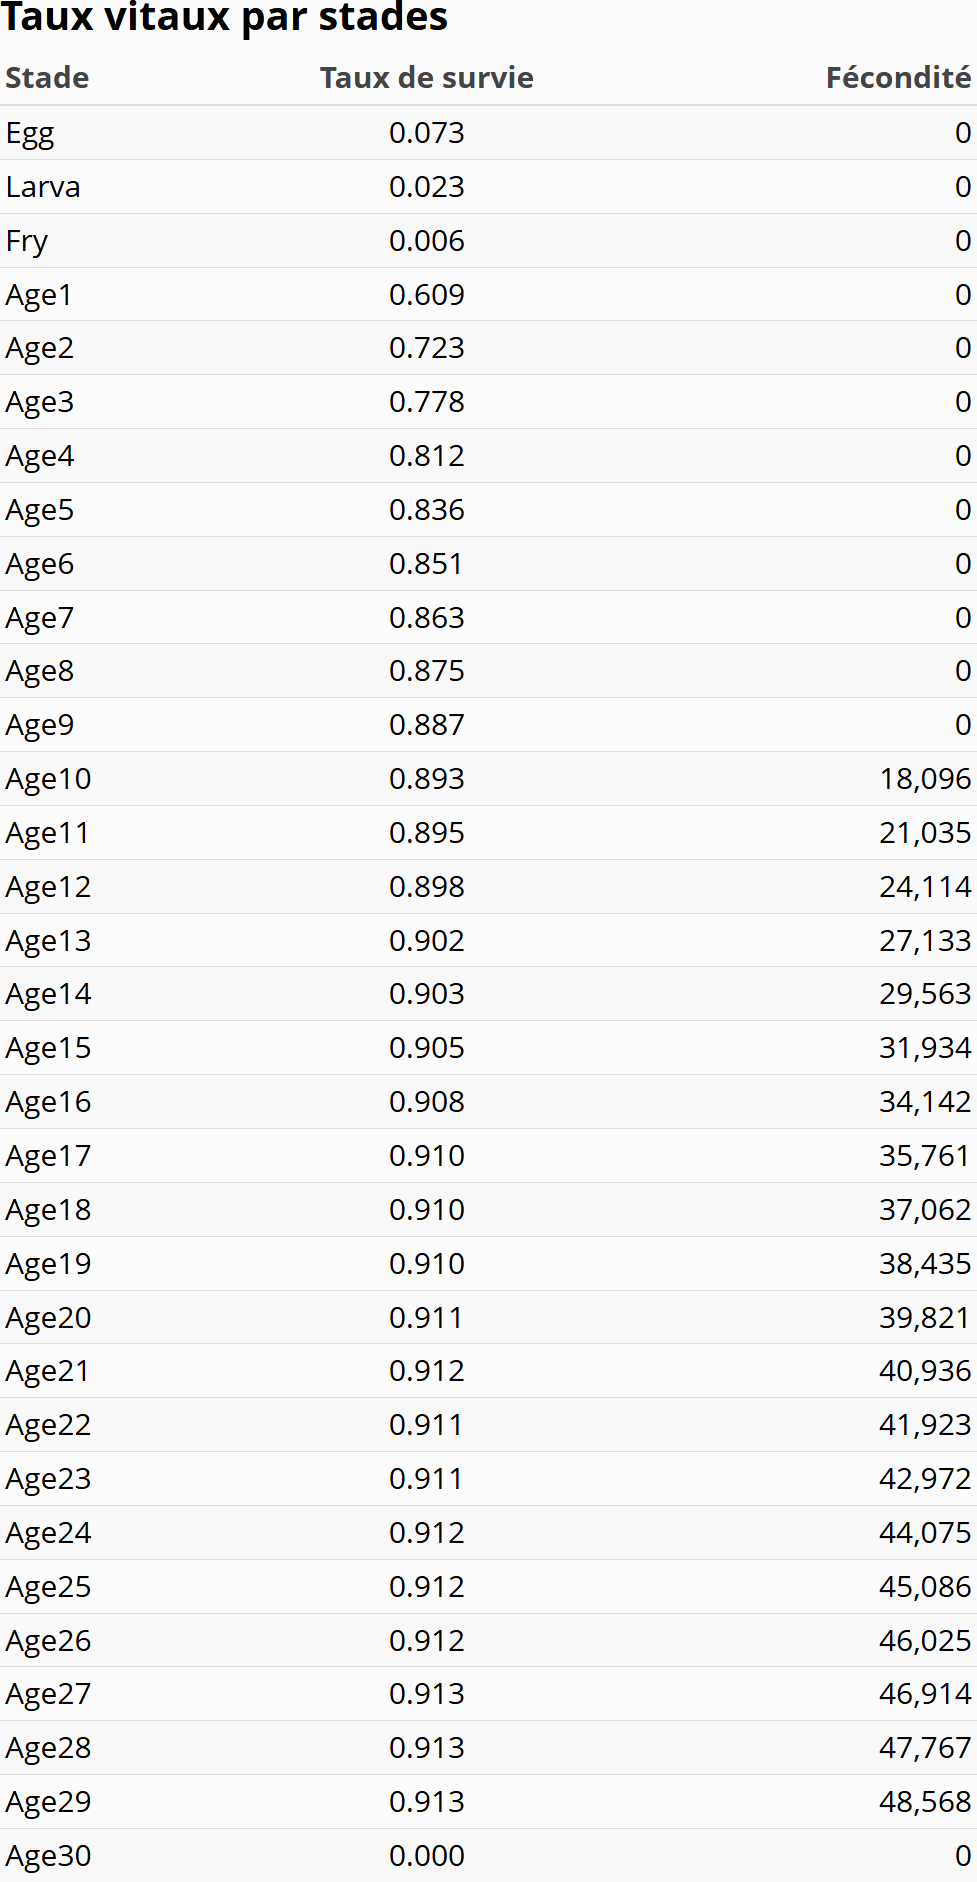
\includegraphics[width=0.5\linewidth,height=\textheight,keepaspectratio]{images/population_table.png}
\caption{Données utilisées pour la matrice mesurée. Sont représentés :
le stade, le taux de survie (valeur de la sous-diagonale de la matrice
de Leslie) et la fécondité (valeur de la première rangée de la matrice
de Leslie)}
\end{figure}

\subsubsection*{Agrégation}\label{agruxe9gation}
\addcontentsline{toc}{subsubsection}{Agrégation}

Pour réduire la complexité du modèle vers une matrice de Lefkovitch à
trois stades, les stades intra-annuels de la matrice originale (« eggs
», « larvae » et « fry ») ont été combinés en un premier stade nommé «
Juvéniles ». Les stades 4 à 13, correspondant aux individus adultes non
reproducteurs, ont été agrégés pour former le stade « Pré-adultes ».
Enfin, les stades 14 à 33, regroupant les individus matures, forment le
stade « Adultes ».

Afin de préserver les dynamiques d'élasticité du modèle original, nous
avons appliqué la méthode d'agrégation décrite par Hinrichsen, Yokomizo,
and Salguero-Gómez (2026). La dynamique initiale est formulée sous forme
matricielle :

\[
x(t+1) = Ax(t)
\]

\noindent où \(x(t)\) est la distribution des individus par classe d'âge
au temps \(t\) et \(A\) est la matrice de Leslie (\(n \times n\)). La
projection vers la structure agrégée \(y(t)\) repose sur une matrice de
partition \(P\) (\(m \times n\)) :

\[
y(t) = Px(t)
\] La matrice agrégée \(\hat{B}\) (\(m \times m\)) est ensuite
construite selon :

\[
\hat{B} = PA^kQ
\]

\noindent où \(k\) représente le temps de résidence dans le stade et
\(Q\) est une matrice de poids d'agrégation définie par :

\[
Q = WP^\top(PWP^\top)^{-1}
\] \noindent où \(W = \text{diag}(w)\) correspond à la distribution
stable des âges (vecteur propre dominant de \(A\)). Cette approche
permet de conserver le taux de croissance asymptotique \(\lambda\) ainsi
que les propriétés de sensibilité du modèle initial (Hinrichsen 2023).

\subsubsection*{Stochasticité et
Variabilité}\label{stochasticituxe9-et-variabilituxe9}
\addcontentsline{toc}{subsubsection}{Stochasticité et Variabilité}

Dans l'étude de Bannester-Marchand et al. (2025), la fécondité comporte
une part de variabilité stochastique. Cette stochasticité a été ajoutée
en supposant que la fécondité annuelle des individus variait selon une
loi normale ayant une moyenne (\(\mu\)) de 0 et un écart-type
(\(\sigma\)) de 0,25. Ainsi, la fécondité des individus varie entre
aucun œuf par année jusqu'au double de la moyenne annuelle.
Contrairement à l'approche de Bannester-Marchand et al. (2025), où
chaque classe d'âge possédait une variabilité indépendante, la présente
étude applique une variabilité annuelle synchrone à l'ensemble du stade
« Adultes ». Cette décision repose sur une logique biologique : les
individus reproducteurs d'une même population sont soumis aux mêmes
fluctuations environnementales. Étant donné que l'espèce est restreinte
à une aire de répartition limitée et à seulement deux sites de fraie
connus, il est plus réaliste de modéliser une réponse commune de la
fécondité face aux conditions annuelles.

Pour les taux de survie, nous avons suivi la méthode de
Bannester-Marchand et al. (2025) en utilisant une distribution bêta. Le
paramètre \(\alpha\) est défini comme suit : \[
\frac{s_{stade} \times \beta}{1 - s_{stade}}
\] \noindent où \(s_{stade}\) est la survie du stade et \(\beta\)
représente la variabilité. Nous avons sélectionné les valeurs de
Bannester-Marchand et al. (2025) offrant la plus grande variabilité,
soit \(\beta = 5,05\) pour les Juvéniles et \(\beta = 0,75\) pour les
Pré-adultes. Pour les probabilités de rester dans un stade, les valeurs
de \(\beta\) ont été ajustées (1 et 0,75) afin d'assurer que la somme de
la survie et de la stase demeure biologiquement cohérente (inférieure ou
égale à 1).

\subsubsection*{Modélisation}\label{moduxe9lisation}
\addcontentsline{toc}{subsubsection}{Modélisation}

Le modèle de viabilité des populations (PVA) a été simulé sur
\(N = 5000\) itérations pour une période de \(t = 100\) ans. La
probabilité d'extinction est définie par l'atteinte d'une abondance
nulle :

\[
P_{ext} = P(\exists t \in [0, 100] : n_{total}(t) = 0)
\] \noindent Nous avons également évalué la probabilité que l'abondance
des individus matures (\(n_{mat}\)) se maintienne au-dessus de seuils
critiques \(k\) (0 et 1000 individus) pour favoriser la diversité
génétique :

\[
P(n_{mat}(t) > k), \quad \forall t \in [0, 100] \text{ où } k \in \{0, 1000\}
\] Enfin, nous avons testé l'efficacité des ensemencements pour
atteindre une cible de 5000 individus matures. Bien que l'analyse
utilise la matrice agrégée à trois stades, les taux de survie
spécifiques aux stades ensemencés (larves, alevins, individus d'un an et
de dix ans) ont été maintenus identiques à ceux de Bannester-Marchand et
al. (2025) pour garantir la comparabilité des stratégies d'intervention.

\section*{Résultats}\label{ruxe9sultats}
\addcontentsline{toc}{section}{Résultats}

\begin{figure}
\centering

\includegraphics[width=1\linewidth,height=1\textheight]{images/fig_2_3.png}
\caption{Résultats de notre analyse. Est représenté : Abondance médiane
de chevaliers cuivrés, basée sur 5000 itérations stochastiques pour les
scénarios (a) nul, (b) menacé, (c) mesuré de notre modèle dynamique. Les
enveloppes colorées représentent les intervalles de confiance à 95\% ;
les lignes pleines les abondances médianes d'individus matures.}
\end{figure}

\indent Les simulations stochastiques indiquent un déclin démographique
dans l'ensemble des scénarios testés. Le scénario « mesuré » (c) montre
l'effondrement le plus rapide, avec une abondance d'individus matures
devenant résiduelle après seulement quelques décennies. Bien que les
scénarios « menacé » (b) et « nul » (a) ralentissent la vitesse de
déclin, la tendance à la baisse demeure constante au fil du temps. Une
forte variabilité inter-simulations est observée, comme en témoignent
les larges intervalles de confiance, soulignant l'impact prépondérant de
la stochasticité sur la dynamique de l'espèce, bien que celle-ci soit
plus faible que celle observée dans Bannester-Marchand et al. (2025).
Malgré cette incertitude, les médianes convergent vers une conclusion
identique : la population ne parvient pas à se maintenir à long terme.
On observe que les différences entre scénarios changent surtout la
vitesse du déclin, mais pas la tendance générale, ce qui suggère que les
paramètres de survie et la structure du modèle contrôlent fortement la
dynamique.

\begin{figure}
\centering

\includegraphics[width=1\linewidth,height=1\textheight]{images/figure3_3.png}
\caption{Résultats de notre analyse. Est représenté : Les probabilités
que les chevaliers cuivrés tombent sous un seuil de population dans les
prochaines 100 ans, basé sur nos scénarios dynamique stochastiques de
population. Lignes : médiane de 5000 itérations; enveloppes colorées :
70\% ICs}
\end{figure}

Les probabilités de passer sous des seuils critiques augmentent
rapidement (Figure 3). La probabilité que la population mature chute
sous la barre des 1000 individus devient élevée dans tous les scénarios,
y compris pour le scénario « nul ». Ainsi, même sous les hypothèses les
plus optimistes, le maintien d'une population viable à long terme
apparaît peu probable sans intervention majeure.

\begin{figure}
\centering

\includegraphics[width=1\linewidth,height=1\textheight]{images/figure4_3.png}
\caption{Résultats de notre analyse. Est représenté : L'effet
d'augmenter l'ensemencement de larves, alevins, individus d'âges 1, et
individus matures (âge 10) sur l'abondance de chevaliers matures sur 100
ans dans notre scénario mesuré.}
\end{figure}

Les simulations d'ensemencement révèlent que des apports massifs sont
nécessaires pour atteindre une cible de 5000 individus matures après un
siècle.Si l'augmentation du nombre d'individus introduits accroît
l'abondance finale, cette relation n'est pas proportionnelle. Notamment,
les ensemencements réalisés à des stades de vie plus avancés (individus
d'un an ou matures) présentent une efficacité nettement supérieure à
ceux effectués aux stades larvaires ou d'alevins (Figure 4).

\section*{Discussion}\label{discussion}
\addcontentsline{toc}{section}{Discussion}

\indent Nos résultats diffèrent de ceux obtenus par Bannester-Marchand
et al. (2025). Dans tous les scénarios testés, les populations simulées
avec la matrice de Lefkovitch à trois stades tendent à s'effondrer plus
rapidement. De plus, même une augmentation massive des ensemencements ne
parvient pas à maintenir une abondance élevée d'individus matures à long
terme. Ces observations suggèrent que notre modèle simplifié offre une
vision plus pessimiste de la dynamique de la population.

\indent Cette divergence s'explique probablement par la simplification
structurelle du modèle. Le passage de 33 stades à seulement trois
entraîne une perte substantielle d'information sur les transitions entre
les classes d'âge. Bien que la méthode d'agrégation utilisée permette de
conserver certaines propriétés asymptotiques, comme le taux de
croissance (\(\lambda\)), elle ne capture pas nécessairement les
dynamiques transitoires à court et moyen terme. Or, ces dynamiques sont
cruciales dans une analyse de viabilité des populations (PVA),
particulièrement lorsque l'effectif est faible et sensible aux
fluctuations.

Le traitement de la stochasticité peut aussi expliquer les différences
observées. Dans notre modèle, la fécondité varie de façon synchrone pour
l'ensemble des adultes, alors que Bannester-Marchand et al. (2025)
appliquaient une variabilité indépendante entre les classes d'âge. Ce
choix amplifie les fluctuations annuelles : concrètement, une année
environnementale défavorable affecte simultanément tous les
reproducteurs, ce qui peut accélérer le déclin démographique. À cet
égard, il serait pertinent de tester différentes approches de
modélisation de la stochasticité. L'absence de consensus dans la
littérature sur la méthode optimale pour combiner les variabilités
inter-stades lors d'une agrégation constitue une limite ici explorée ;
une paramétrisation plus fine, appuyée par une expertise accrue en
dynamique stochastique, permettrait potentiellement de converger
davantage vers les résultats du modèle détaillé.

Les résultats obtenus montrent également que l'ensemencement, tel qu'il
est modélisé ici, ne suffit pas à assurer la viabilité de la population.
L'augmentation du nombre de larves ou d'alevins n'a pas l'impact
escompté sur l'abondance des adultes à long terme. Cela souligne le rôle
critique des stades juvéniles et pré-adultes : si la survie à ces étapes
de vie est trop faible, le recrutement vers le stade adulte demeure
insuffisant, quel que soit l'effort d'introduction initial. Par
conséquent, des mesures visant à améliorer les conditions de survie
(restauration de l'habitat, qualité de l'eau, accès aux frayères)
pourraient s'avérer plus efficaces qu'une simple intensification des
ensemencements.

Malgré ces différences, les tendances générales demeurent cohérentes
avec les connaissances actuelles sur l'espèce. La population reste
extrêmement vulnérable et dépendante des interventions humaines. La
difficulté à maintenir une population stable sans soutien artificiel
confirme le statut précaire du Chevalier cuivré.

En conclusion, cette étude met en évidence les limites inhérentes aux
modèles simplifiés. Si la matrice de Lefkovitch à trois stades est plus
parcimonieuse et exige moins de données, elle introduit des biais
importants qui, dans ce cas précis, semblent accentuer le déclin de la
population. Bien que ce type de modèle soit utile pour explorer
rapidement divers scénarios, il doit être utilisé avec prudence. Pour
des analyses de viabilité plus précises, le maintien d'une structure
d'âge détaillée demeure essentiel.

\section*{Bibliographie}\label{bibliographie}
\addcontentsline{toc}{section}{Bibliographie}

\pnasbreak

\phantomsection\label{refs}
\begin{CSLReferences}{1}{0}
\bibitem[\citeproctext]{ref-bannester-marchand_population_2025}
Bannester-Marchand, N, N Vachon, Ne Mandrak, and Fg Blanchet. 2025.
{``Population Viability Analysis of the Endangered Copper Redhorse
\emph{{Moxostoma} Hubbsi}.''} \emph{Endangered Species Research} 57
(May): 21--31. \url{https://doi.org/10.3354/esr01395}.

\bibitem[\citeproctext]{ref-cosepac_evaluation_2014}
COSEPAC. 2014. {``Évaluation Et {Rapport} de Situation Du {COSEPAC} Sur
Le Chevalier Cuivré (\emph{{Moxostoma} Hubbsi}) Au {Canada}.''}
\emph{Comité Sur La Situation Des Espèces En Péril Au Canada}, xiii +
81.
\url{https://wildlife-species.canada.ca/species-risk-registry/virtual_sara/files/cosewic/sr_Copper\%20Redhorse_2014_f.pdf}.

\bibitem[\citeproctext]{ref-dahlberg_review_1979}
Dahlberg, Michael D. 1979. {``A Review of Survival Rates of Fish Eggs
and Larvae in Relation to Impact Assessments.''} \emph{Marine Fisheries
Review} 41 (3).

\bibitem[\citeproctext]{ref-hinrichsen_aggregation_2023}
Hinrichsen, Richard A. 2023. {``Aggregation of {Leslie} Matrix Models
with Application to Ten Diverse Animal Species.''} \emph{Population
Ecology} 65 (3): 146--66. \url{https://doi.org/10.1002/1438-390X.12149}.

\bibitem[\citeproctext]{ref-hinrichsen_theory_2026}
Hinrichsen, Richard A., Hiroyuki Yokomizo, and Roberto Salguero-Gómez.
2026. {``From Theory to Application: {Elasticity}-Consistent Aggregation
of {Leslie} Matrix Population Models for Comparative Demography.''}
bioRxiv. \url{https://doi.org/10.64898/2026.02.04.703802}.

\bibitem[\citeproctext]{ref-mongeau_biologie_1986}
Mongeau, Jean-René, Pierre Dumont, and Louise Cloutier. 1986. \emph{La
Biologie Du {Suceur} Cuivré, \emph{{Moxostoma} Hubbsi}, Une Espèce Rare
Et Endémique à La Région de {Montréal}, {Québec}, {Canada}}.
\url{https://portals.iucn.org/library/node/15279}.

\bibitem[\citeproctext]{ref-mongeau_biologie_1992}
---------. 1992. {``La Biologie Du Suceur Cuivré (\emph{{Moxostoma}
Hubbsi}) Comparée à Celle de Quatre Autres Espèces de \emph{Moxostoma}
(\emph{{M}. Anisurum, {M}. Carinatum, {M}. Macrolepidotum} Et \emph{{M}.
Valenciennesi}).''} \emph{Canadian Journal of Zoology} 70 (7): 1354--63.
\url{https://doi.org/10.1139/z92-191}.

\bibitem[\citeproctext]{ref-vachon_recherche_2020}
Vachon, Nathalie. 2020. \emph{Recherche de Subadultes Du Chevalier
Cuivré Et Suivi Du Recrutement En 2016}.
\url{https://doi.org/10.13140/RG.2.2.33614.79689}.

\bibitem[\citeproctext]{ref-vachon_reproduction_2021-1}
---------. 2021a. \emph{Reproduction Artificielle, Ensemencements Et
Suivi de La Population Du Chevalier Cuivré (\emph{{Moxostoma} Hubbsi})
En 2018}.

\bibitem[\citeproctext]{ref-vachon_reproduction_2021-2}
---------. 2021b. {``Reproduction Artificielle, Ensemencements Et Suivi
de La Population Du Chevalier Cuivré (\emph{{Moxostoma} Hubbsi}) En
2019.''}
\url{https://www.researchgate.net/publication/356970163_Reproduction_artificielle_ensemencements_et_suivi_de_la_population_du_chevalier_cuivre_Moxostoma_hubbsi_en_2019}.

\end{CSLReferences}



% Bibliography
% \bibliography{pnas-sample}

\end{document}
